\chapter{风格迁移,创作属于你的名画}

\section{风格迁移的前世今生}

风格图像迁移指的是讲图像A的风格转换到图像B中,得到新的图像。其开山之作为《Image style transfer using convolutional neural networks》\cite{gatys2016image}。然后在短短的一段时间内,世界范围内的研究者在风格迁移领域发表了大量的论文,其中经典的一篇论文是名为《Perceptual losses for real-time style transfer and super-resolution》\cite{johnson2016perceptual}。

\section{什么是风格}
\subsection{Gram矩阵描述风格}
\begin{newdef}[Gram矩阵]
$n$维欧式空间中任意$k(k\leq n)$个向量$\alpha_1$,$\alpha_2$,$\ldots$,$\alpha_k$的内积所组成的矩阵
\begin{equation*}
\bigtriangleup (\alpha_1,\alpha_2,\ldots,\alpha_k) = 
\left(
\begin{array}{cccc}
(\alpha_1,\alpha_1) & (\alpha_1,\alpha_2) & $\ldots$ & (\alpha_1,\alpha_k) \\ (\alpha_1,\alpha_1) & (\alpha_1,\alpha_2) & $\ldots$ & (\alpha_1,\alpha_k) \\
$\ldots$ & $\ldots$ & $\ldots$ & $\ldots$ \\
(\alpha_1,\alpha_1) & (\alpha_1,\alpha_2) & $\ldots$ & (\alpha_1,\alpha_k) \\
\end{array}
\right)
\end{equation*}
称为$k$个向量$\alpha_1$, $\alpha_2$,$\ldots$,$\alpha_k$的格拉姆矩阵(Gram矩阵),它的行列式称为Gram行列式。
\end{newdef}

Gram矩阵可以看做特征之间的偏心协方差矩阵(即没有减去均值的协方差矩阵),在特征图中,每个数字都来自于一个特定滤波器在特定位置的卷积,因此每个数字代表一个特征的强度,而Gram计算的实际上是两两特征之间的相关性,哪两个特征是同时出现的,哪两个是此消彼长的等等,同时,Gram的对角线元素,还体现了每个特征在图像中出现的量,因此,Gram有助于把握整个图像的大体风格。由此产生了表示风格的Gram矩阵,要度量两个图像风格的差异,只需比较他们Gram矩阵的差异即可。

总之, Gram矩阵用于度量各个维度自己的特性以及各个维度之间的关系。内积之后得到的多尺度矩阵中,对角线元素提供了不同特征图各自的信息,其余元素提供了不同特征图之间的相关信息。这样一个矩阵,既能体现出有哪些特征,又能体现出不同特征间的紧密程度。

\subsection{Gram矩阵的应用}

在《Image style transfer using convolutional neural networks》\cite{gatys2016image}出来之前,Gatys还做了这个工作《Texture Synthesis Using Convolutional Neural Networks》~\cite{gatys2015texture},他们发现如果让隐藏层的特征用协方差来进行进行约束,可以得到较好的纹理生成,他们发现如果用协方差(也就是Gram矩阵)来进行约束隐藏层特征的话,重建出来的特征虽然有些会保持,但是有些可能位置会打散。比如最右侧的一张图,人还是人,但是重建出来相当于“拼图”效果了。这是因为协方差本身就是去除了位置信息。 那么既然协方差可以用于纹理生成,那么如果我们加上 “让生成图的隐藏层特征与原图尽量一样,另一方面让生成图的打散特征与画的打散特征尽量相似”,这就是用神经网络做风格转换的最初想法。这也比较符合“风格”的定义,毕竟风格不应该具有位置信息,一种风格应该是与位置无关的。

\begin{figure}[hbtp]
  \centering
  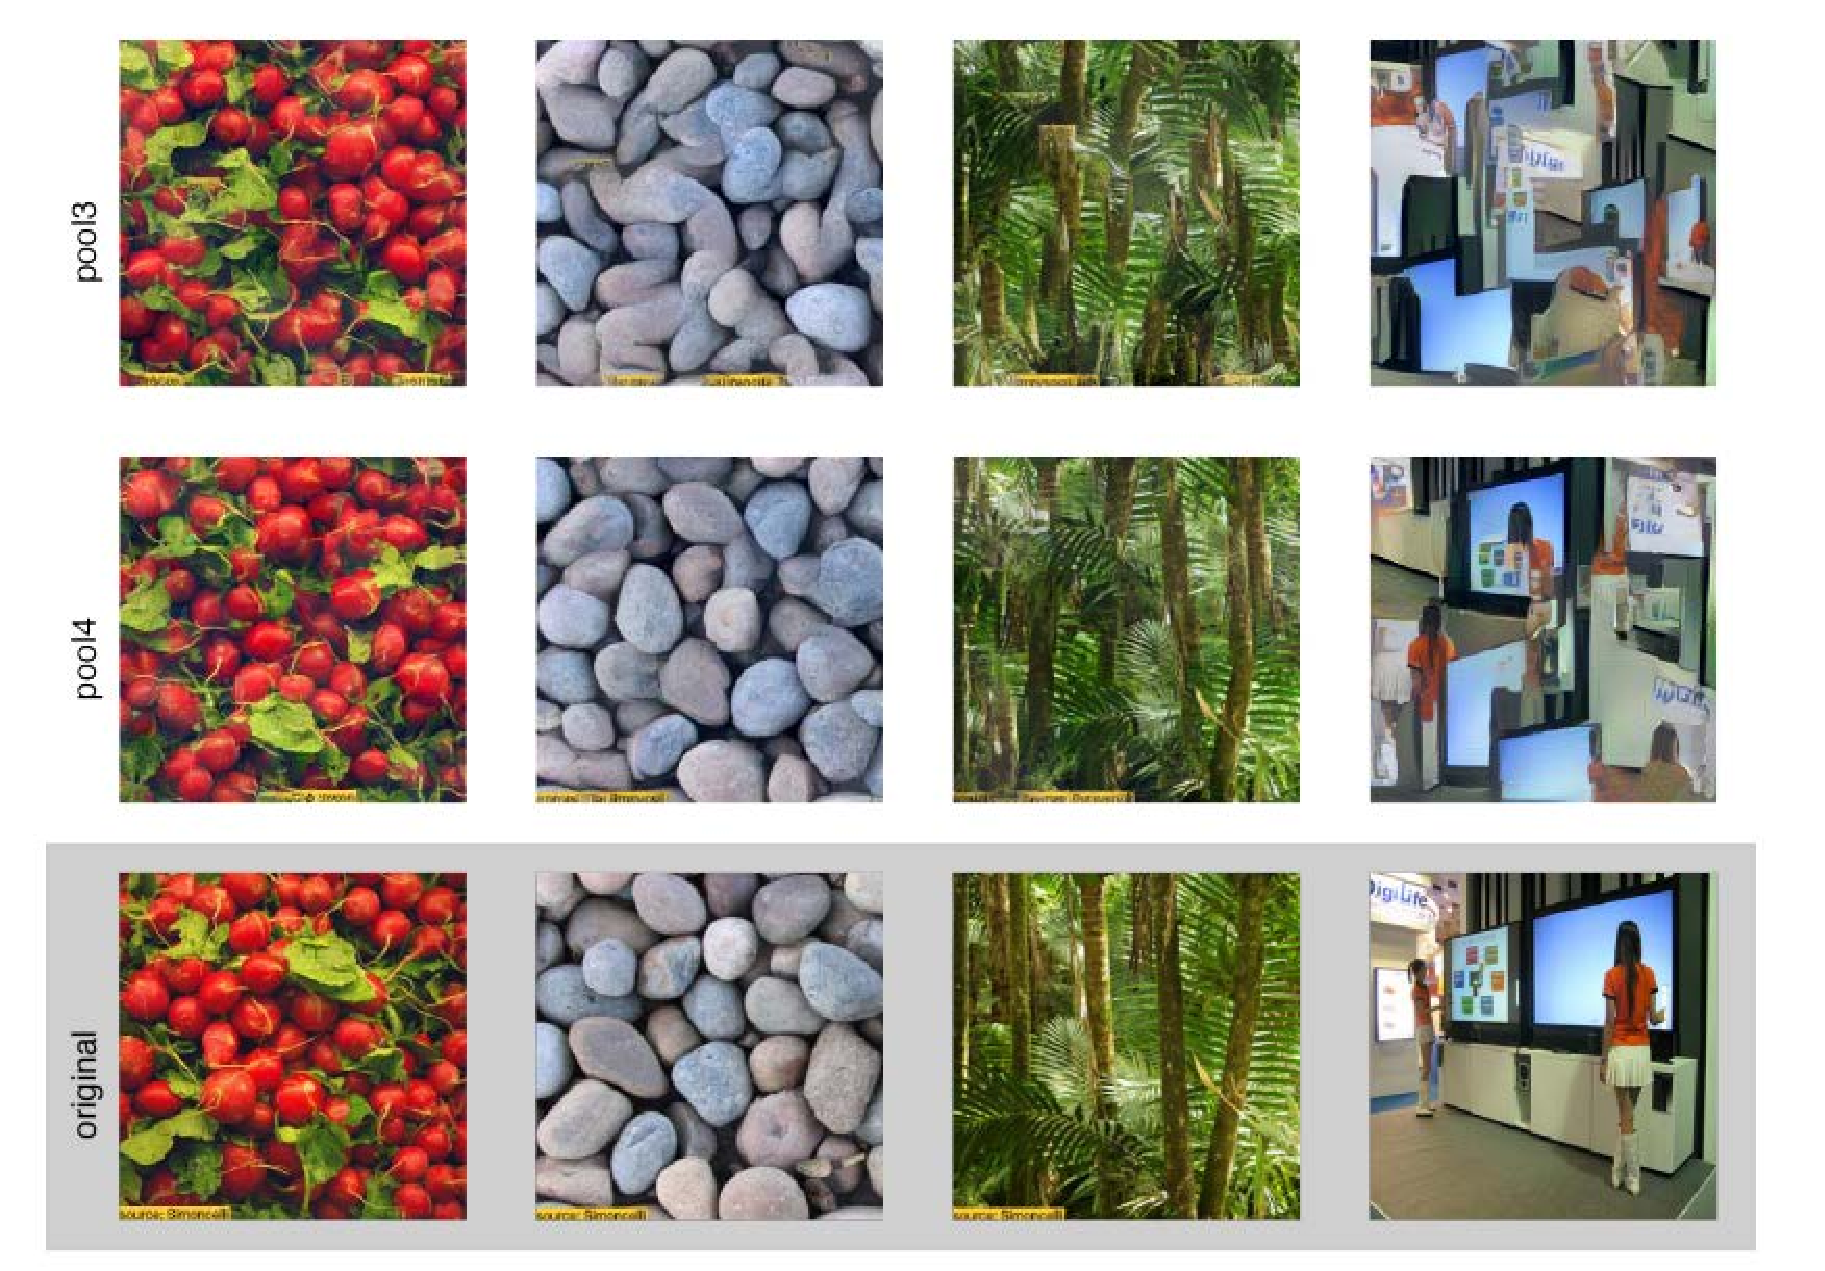
\includegraphics[width=0.8 \linewidth]{image/style_transfer/texture.pdf}
  \caption{纹理}
  \label{fig:texture}
\end{figure}

需要注意的是Gatys的几篇论文没有解释为什么用Gram矩阵, 其实可以这样认为, 协方差就是一种二阶统计信息, 我们要求输出图的什么信息与风格图相近, 肯定不是特征图上单纯的逐点的相近, Gram矩阵描述的就是全局特征的自相关, 如果输出图与风格图的这种自相关相近, 那么差不多是我们所理解的”风格”。 当然,其实也可以用很多其他的统计信息进行描绘风格。 这也就是后面有用直方图的, 甚至直接简化成”均值+方差”进行描绘风格的。

\section{通过深度学习进行风格迁移}

下面约定$p$为风格图,$a$为待转换的图,即内容图。比如$p$为某张梵高的画,$a$为某个场景,生成为 $f$,即具有梵高的画的风格的场景图。首先定义两个损失, $l_{style}$和$l_{content}$,前者希望$f$和$p$在“风格”上尽量一致,后者则希望$f$与$a$在内容上尽量一致。
\begin{equation}
\label{eq:transfer_loss}
  l(a,f,p)=\alpha \ast l_{style}(p,f) + \beta \ast l_{content}(a,f)
\end{equation}

其中,公式~\ref{eq:transfer_loss}的$\alpha$和$\beta$为两个损失的平衡参数。我们希望$l$尽量小,采用梯度下降即可优化。所用的CNN网络是VGG-19。开始训练时,随机生成 $a$同等大小的随机噪声图 $x$,通过指定不同的层作为content损失的提取层$L_c$ 以及style损失的提取层$L_s$,使得$x$在$L_c$层得到的内容损失 $l_{content}(L_c,x)$与$l_{content}(L_c,a)$尽量一样。同时,使得 $x$在 $L_s$层得到的风格损失$l_{style}(Ls,x)$与 $l_{style}(L_s,p)$也尽量一样。其中$l_{content}$的具体形式可以由MSE来指定,而 $l_{stylel}$可由对应的Gram矩阵来计算。

\section{总结}

\bibliographystyle{ieeetr}
\bibliography{reference}
\addcontentsline{toc}{section}{参考文献}